\begin{quote}
  We develop a structured prediction approach to reconstructing 3D
  polygonal models from single and multiple images of a
  scene. Building on recent advances in single view reconstruction we
  adopt the indoor Manhattan hypothesis class --- one of the most
  complicated output spaces (in terms of internal constraints) yet
  considered within a structured prediction framework. Our approach
  can learn in both the single-- and multiple--view contexts. We
  show that the chosen hypothesis class permits optimising a variety
  of high--level loss functions, such as the relative depth error. Our
  results out--perform the state--of--the--art, including an
  improvement of more than $50\%$ on one metric.\footnotemark
\end{quote}

\footnotetext{At the time of publishing, part of the work presented in
  this chapter was under review for the 2012 European Conference on
  Computer Vision.}

\section{Introduction}
\label{sec:introduction}

Previous chapters cast scene understanding as a fixed inference
problem, with each input instance considered separately. Such systems
have no capacity to improve their accuracy over time based on feedback
from past predictions, since there is no information carried over from
one inference task to the next. This chapter considers the task of
learning to recover indoor Manhattan models based on labelled training
examples. We are given a series of input images together with ground
truth reconstructions, and the goal is to discover a rule to recover
the correct scene structure from future images.

We adopt the standard approach in machine learning of distinguishing a
learning phase --- a one--off computation performed ahead of time ---
from the inference phase --- in which the results of the learning
phase are used to label incoming training examples. This chapter
focusses on the learning phase; we will show that under the learning
scheme we propose, inference reduces to exactly the algorithm
presented in the previous chapter. As a result, the approach described
in this chapter is strictly complimentary to the inference algorithm
described in \chapref{inference}.

In this chapter we emphasise a learning--based approach to recovering
scene structure. Traditionally, neither the single-- nor
multiple--view reconstruction literature places learning at the heart
of the reconstruction problem. Within single--view reconstruction, for
example, few authors cast learning as a single optimisation with
respect to a clearly defined loss function
\cite{Hoiem05,Saxena09,Lee09,Flint11}. On the other hand,
multiple--view reconstruction techniques rarely learn from training
data at all. In contrast, this chapter casts reconstruction
fundamentally as a learning problem, with the goal being to learn a
prediction function $\Predictor$ mapping observed image features to
indoor Manhattan reconstructions.

Using indoor Manhattan reconstructions as the hypothesis class brings
a variety of attractive features such as a simple parametrisation,
efficient and exact inference, and a balance between expressiveness
and robustness, as has been discussed in preceding chapters. In this
chapter we show that this hypothesis class also leads to a convenient
decomposition of loss functions mirroring the likelihood decomposition
described in \chapref{inference}, which permits efficient optimisation of
several popular image--level losses.

For learning we employ the tools of structured prediction --- in
particular, the structured support vector machine
\cite{Tsochantaridis04}. The use of these tools is part of a long
trend within computer vision towards statistically rigorous,
well--understood convex optimisation techniques. Recent successfully
applications of the structured SVM include detection
\cite{blaschko2008learning}, segmentation \cite{taskar2004max}, and
scene classification \cite{Yang2010}. In the domain of reconstruction,
structured prediction ideas have been applied to several simple models
classes such as stereo disparities \cite{li2008learning} and cuboids
\cite{Hedau09}.

The application of structured prediction to the indoor Manhattan class
of models constitutes one of the most complex output spaces yet
considered within this framework. The indoor Manhattan model enforces
hard geometric constraints that lack simple expressions in terms of
individual pixel labels. These constraints are time--varying,
being tied to quantities such as camera rotation and the location of
vanishing points. We have learnt several valuable lessons of general
relevance from this complex prediction task, to which we dedicate the
final section of this chapter.

The contributions of this chapter are thus (i) a unified learning
framework for single-- and multiple--view reconstruction, utilising
the indoor Manhattan model and the tools of structured prediction;
(ii) the reduction of two image--level loss functions to a form
amenable to efficient optimisation; (iii) an efficient separation
procedure for identify the ``most--violated constraint'' during
learning, (iv) an empirical demonstration of structured prediction in
perhaps the most complex output space yet considered within this
framework; and (v) a series of practical observations concerning the
application of structured prediction techniques to complicated output
spaces.

\section{Background}

\newcommand\inp{\vect{x}}
\newcommand\outp{\vect{y}}

The approach to learning adopted in this chapter has roots in the
structural risk minimisation framework developed by Vapnik and
Chervonenkis \cite{Vapnik1998}. On this view, learning is framed in
terms of a predictor $\Predictor$, which maps from an input space
$\mathcal{X}$ to an output space $\mathcal{Y}$. Learning consists of
minimising the expected loss
\begin{equation}
  \label{eq:expected-utility-maximization}
  \Expected\bigl[ \Loss(f(\inp),\outp) \bigr] 
  =
  \int \Loss\bigl(\Predictor(\inp),\outp\bigr) ~ \intd P(\inp,\outp)
\end{equation}
with respect to the predictor $\Predictor$, where $\Loss$ is a loss
function. Given training samples
$(\inp_i,\outp_i)\in\mathcal{X}\cross\mathcal{Y}$, the integral above
is approximated by\changedsinceviva
\begin{equation}
  \label{eq:erm}
  \sum_i \Loss\bigl(\Predictor(\inp_i),\outp_i\bigr)~.
\end{equation}
Structural risk minimisation techniques add a regulariser
$\mathcal{R}$, yielding\changedsinceviva
\begin{equation}
  \label{eq:srm}
  \mathcal{R}(\Predictor) + \sum_i \Loss\bigl(\Predictor(\inp_i),\outp_i\bigr)
\end{equation}
Structural risk minimisation does not specify any particular form for
the input space, output space, predictor class, or loss function. Many
machine learning algorithms can be viewed as instantiations of
structural risk minimisation for particular predictor classes and loss
functions. For example, the classic support vector machine (SVM)
\cite{Cortes1995} is defined for Hilbert input spaces, binary output
spaces, the hypothesis class of linear predictors, and the Hinge loss
function. In this case equation \eqnref{srm} becomes
\begin{equation}
  \|\Model\|^2 + \sum h(\outp_i, \Model \cdot \inp_i))
\end{equation}
where $h$ is the hinge loss, and learning consists of minimisation
with respect to $\Model$. Rewriting the hinge loss as a soft
constraint leads to the well--known quadratic programming formulation
of the SVM \cite{Cortes1995}.

Extending binary classification to more general output spaces is a
major research programme within machine learning; an excellent
introduction to recent advances is given by Bakir \etal
\cite{Bakir07}. One recently successful approach is the structured
support vector machine proposed by Tsochantaridis \etal
\cite{Tsochantaridis04}, which reduces learning in non--binary
(``structured'') output spaces to a ranking problem. The structured
SVM makes use of a joint feature space $\JointFtr(\inp,\outp)$ mapping
input/output pairs to real vectors. The hypothesis class consists of
predictors of the form
\begin{equation}
  \Predictor(\inp;\Model) 
  = 
  \argmax_{\outp}\limits 
  \bigl\langle \Model, \JointFtr(\inp,\outp) \bigr\rangle
  \label{eq:linear-max}
\end{equation}
where $\Model$ is a parameter vector and $\langle\cdot,\cdot\rangle$
denotes an inner product. As in the classic SVM, the hinge loss is
used to define the objective function,
\begin{equation}
  \label{eq:first-ssvm}
  \|\Model\|^2 + \sum h(\outp_i, \Predictor(\inp_i)) ~.
\end{equation}
In order to optimise with respect to $\Model$, Toschantaridis \etal
showed how to write \eqnref{first-ssvm} as a constrained optimisation
problem paralleling the classic SVM:
\begin{equation}
  \begin{split}
    \min_{\Model,\Slacks} &
      \hspace{2mm} 
    \frac{1}{2} \|\Model\|^2 +
      C \sum_{i=1}^n \Slack_i\\
    s.t. & \hspace{2mm} 
      \forall k, \outp \neq \outp_i:~
        \bigl\langle\Model, \JointFtr(\inp_i,\outp_i)\bigr\rangle -
        \bigl\langle\Model, \JointFtr(\inp_i,\outp)\bigr\rangle
      \geq
        \Loss(\outp,\outp_i) - \Slack_i ~.
  \end{split}
  \label{eq:ssvm}
\end{equation}
Unfortunately the number of constraints in \eqnref{ssvm} is in general
very large since there is a constraint for every element of the output
space. Tsochantaridis \etal \cite{Tsochantaridis04} showed how to
overcome this by exploiting the sparsity structure of support vector
machines. Their algorithm iteratively adds constraints beginning with
zero constraints, and they showed that only a polynomial number of
constraints need ever be added in order to achieve an
$\epsilon$--accurate solution. The remainder of this chapter shows how
to use the structured SVM to learn to reconstruct indoor Manhattan
models.

\section{Model}
\label{sec:model}

In this section we describe three components of the model that we are
trying to learn (and, at test time, infer): a hypothesis class, a
feature space, and a loss function. In our setup these are,
respectively, the class of indoor Manhattan models, a log--linear
Bayesian likelihood, and either the relative depth error or a
labelling error (we describe both).

\subsection{Hypothesis Class}

This chapter is concerned with the output space consisting of indoor
Manhattan reconstructions as described in \chapref{geometry}. For
consistency with preceding chapters we use the following notation:
our input space consists of observed image features denoted
$\Features$, and the output space consists of indoor Manhattan
reconstructions in the seam representation denoted $\Seam$. A training
sample is then a set of pairs $\{(\Features_i,\Seam_i)\}$.

\subsection{Feature Space}

In order to learn to reconstruct indoor Manhattan models we must
define a family of prediction functions $\Predictor$ mapping image
features to indoor Manhattan models. Building on \chapref{inference},
we would like each predictor to implement MAP inference for some
value of the hyper--parameters, \ie we are interested in predictors of
the form
\begin{equation}
  \label{eq:map-predictor}
  \Predictor(\Features) = 
  \argmax_{\Seam}\limits P(\Seam ~|~ \Features,\Model)
\end{equation}
for various $\Model\in\Reals^n$. In other words, we would like to
optimise over the set
\begin{equation}
  \Bigl\{ 
    \Predictor ~\bigl|~
    \Predictor: \Features \longmapsto 
    \argmax_{\Seam}\limits P(\Seam ~|~ \Features,\Model), \Model\in\Reals^n
  \Bigr\}
\end{equation}
consisting of MAP inference predictors for all possible
hyper--parameter values, which we have grouped into the parameter
$\Model$. In order to employ the structured SVM we need to write
$\Predictor$ in the form \eqnref{linear-max}, or equivalently, we need
to write the logarithm of the posterior on scene structure in the form
\begin{equation}
  \log P(\Seam ~|~ \Features,\Model)
  =
  \bigl\langle \Model, \JointFtr(\Features,\Seam) \bigr\rangle ~.
\end{equation}
That is, we need to show that the posterior described in the previous
chapter is log--linear. The remainder of this section is devoted to
defining a joint feature map $\JointFtr$ permitting such a
representation. We now examine each term in the posterior
\eqnref{full-posterior}, our goal being to show that each is
log--linear in the relevant hyper--parameters.

\subsubsection{Prior}
Recall the log--prior \eqnref{log-scene-prior}, which is repeated
below.
\begin{equation}
  \label{eq:log-scene-prior2}
  \log P(\Seam ~|~ \Penalties) =
    -\log Z +
    n_1\log\PenaltyConc + 
    n_2\log\PenaltyConv + 
    n_3\log\PenaltyOccl~.
\end{equation}
Defining $\Counts=\begin{bmatrix}n_1&n_2&n_3\end{bmatrix}$ we have
\begin{equation}
  \label{eq:linear-prior}
  \log P(\Seam ~|~ \Penalties) 
  =
  \bigl\langle \Penalties, \Counts \bigr\rangle ~~ + O(1) ~.
\end{equation}

\subsubsection{Photometric Likelihood}
Combining \eqnref{photometric-loglik} and \eqnref{pixel-likelihood},
the log likelihood for photometric features that was described in
\chapref{inference} is
\begin{equation}
  \log P(\Features ~|~ \Seam) 
  =
  \sum_i \PixelModel_{\PredictedOrient_i} \cdot \Feature_i ~~ + O(1) ~.
\end{equation}
where the sum is over pixels, and, as defined in \chapref{inference},
$\PredictedOrient_i$ is the orientation predicted by $\Seam$ for pixel
$i$, $\PixelModel_\Orient$ is the model for photometric features given
orientation $\Orient$, and $\Feature_i$ is the feature observed at
pixel $i$. We define
\begin{align}
  \PixelModel =
  \begin{bmatrix}
    \PixelModel_1 \\
    \PixelModel_2 \\
    \PixelModel_3
  \end{bmatrix}
  & \quad &  
  \JointFtr_{\textsf{mono}}(\Features,\Seam) =
  \begin{bmatrix}
    \sum_{i:\PredictedOrient_i=1}\limits \Feature_i \vspace{1mm} \\
    \sum_{i:\PredictedOrient_i=2}\limits \Feature_i \vspace{1mm} \\
    \sum_{i:\PredictedOrient_i=3}\limits \Feature_i
  \end{bmatrix}~.
\end{align}
Finally we can write
\begin{equation}
  \label{eq:linear-photometric-model}
  \log P(\Features ~|~ \Seam) 
  =
  \bigl\langle \PixelModel, \JointFtr_{\textsf{mono}}(\Features,\Seam)
  \bigr\rangle ~~ + O(1) ~.
\end{equation}

\subsubsection{Photo--consistency Likelihood}
The log likelihood for photo--consistency features given by equation
\eqnref{stereo-loglik} is
\begin{equation}
  \label{eq:stereo-loglik2}
  \log P(\Features,\AuxFeatures_1,\ldots,\AuxFeatures_{\NumViews}
            ~|~ \Seam) 
  =
  \sum_i \sum_{k=0}^{\NumViews} 
    \|\Feature_i-\ComputedAuxFeature_k(\Pixel_i;\Seam)\|_{\StereoCov} ~.
\end{equation}
Here we assume that
\begin{equation}
  \StereoCov^{-1} = \diag(\StereoCoef_1,\ldots,\StereoCoef_2) ~.
\end{equation}
It follows that by defining
\begin{align}
  \StereoModel =
  \begin{bmatrix}
    \StereoCoef_1 \\
    \vdots \\
    \StereoCoef_m
  \end{bmatrix}
  & \quad &  
  \JointFtr_{\textsf{stereo}}(\Features,\Seam) =
  \begin{bmatrix}
    \sum_i \sum_{k=1}^K \bigl(
      (\Feature_i)_1 - (\ComputedAuxFeature_k(\Pixel_i;\Seam))_1
    \bigr)^2\\
    \vdots \\
    \sum_i \sum_{k=1}^K \bigl(
      (\Feature_i)_m - (\ComputedAuxFeature_k(\Pixel_i;\Seam))_m
    \bigr)^2
  \end{bmatrix}
\end{align}
we can write the log likelihood \eqnref{stereo-loglik2} in the form
\begin{equation}
  \label{eq:linear-stereo-model}
  \log P(\Features,\AuxFeatures_1,\ldots,\AuxFeatures_{\NumViews})
  =
  \bigl\langle
    \StereoModel, \JointFtr_{\textsf{stereo}}(\Features,\Seam)
  \bigr\rangle ~~ + O(1) ~.
\end{equation}

\subsubsection{Point Cloud Likelihood}

The log--likelihood for point cloud features \eqnref{3d-likelihood} is
non--linear so for the purpose of learning we approximate it by a
first order Taylor expansion about $\IndModelo$ as follows.
\begin{eqnarray}
  \log P(\Depth~|~\Seam,\IndModel)
  &\approx&
  \frac
      {\sum_{\Ind} P(\Depth~|~\Seam,\Ind) P(\Ind~|~\IndModel)}
      {\sum_{\Ind} P(\Depth~|~\Seam,\Ind) P(\Ind~|~\IndModelo)} + O(1)\\
  \log P(\Depths~|~\Seam,\IndModel)
  &\approx&
  \sum_i \sum_{\Ind} \frac
      {P(\Depth_i~|~\Seam,\Ind) P(\Ind~|~\IndModel)}
      {\sum_{\Ind} P(\Depth_i~|~\Seam,\Ind_i) P(\Ind~|~\IndModelo)} + O(1) ~.
\end{eqnarray}
It follows that by defining
\begin{equation}
  \JointFtr_{\textsf{3D}}(\Depths,\Seam) =
  \frac{1}{\sum_{\Ind} P(\Depth_i~|~\Seam,\Ind) P(\Ind~|~\IndModelo)}
  \begin{bmatrix}
    \sum_i P(\Depth_i~|~\Seam,\Ind=\IN) P(\Ind=\IN~|~\IndModel) \\
    \sum_i P(\Depth_i~|~\Seam,\Ind=\OUT) P(\Ind=\OUT~|~\IndModel) \\
    \sum_i P(\Depth_i~|~\Seam,\Ind=\ON) P(\Ind=\ON~|~\IndModel)
  \end{bmatrix}~.
\end{equation}
we can write
\begin{equation}
  \label{eq:linear-pt-model}
  \log P(\Depths~|~\Seam,\IndModel)
  =
  \bigl\langle
    \IndModel, \JointFtr_{\textsf{3D}}(\Depths,\Seam)
  \bigr\rangle ~~ + O(1) ~.
\end{equation}

\subsubsection{Posterior}

We have now shown that the likelihoods we defined in \chapref{inference}
for each sensor modality are log--linear in the respective
hyper--parameters. Combining equations \eqnref{linear-prior},
\eqnref{linear-photometric-model}, \eqnref{linear-stereo-model},
and \eqnref{linear-pt-model} we have the following linear form for
the log--posterior,
\begin{equation}
  \log P(\Seam ~|~ X, \Model)
  =
  \bigl\langle
    \Model, \JointFtr(\Observations,\Seam)
  \bigr\rangle
  \label{eq:log-linear-posterior}
\end{equation}
where $\Observations$ denotes all observations from all sensor
modalities and we have defined
\begin{align}
  \Model = \begin{bmatrix}
    \Penalties \\
    \PixelModel \\
    \StereoModel \\
    \IndModel
  \end{bmatrix}
  & \quad &
  \JointFtr(\Observations,\Seam) = \begin{bmatrix}
    \Counts \\
    \JointFtr_{\textsf{mono}} \\
    \JointFtr_{\textsf{stereo}} \\
    \JointFtr_{\textsf{3D}}
  \end{bmatrix}~.
\end{align}

\subsubsection{Discussion}

We have shown in the derivations above that the posterior from
\chapref{inference} is log--linear (or can be approximated as such),
so substituting \eqnref{log-linear-posterior} into
\eqnref{map-predictor} we are now interested in predictors of the form
\begin{equation}
  \label{eq:linear-predictor}
  \Predictor(\Features) = 
  \argmax_{\Seam}\limits
  \bigl\langle
    \Model, \JointFtr(\Observations,\Seam)
  \bigr\rangle~.
\end{equation}

One view of this result is that it is a convenient property of our
chosen likelihoods that allows us to efficiently optimise the
hyper--parameters in the graphical models of \chapref{inference} using
learning algorithm that we describe below. However, an alternative
view is that the joint feature map is simply an arbitrary feature
space with no special interpretation attached to any element. Each
element of the feature space simply expands the range of predictors
that can be expressed in the form \eqnref{linear-predictor}, and we
may add whichever features we believe will be helpful for
reconstruction. The fact that our features are derived from a
graphical model is suggestive of their relevance but not absolutely
necessary.

Both views lead to the same learning objective, which is to optimise
$\Model$ with respect to an expected loss over a training set.

\subsubsection{Features}

The precise make--up of the feature space depends on the available
sensor modalities. For our experiments we define separate feature
spaces for the single-- and multiple--view contexts; these are
summarised in \figref{featurespace}.

\begin{table}[tb]
  \centering
  \begin{tabular}{@{}lllll@{}}
    \toprule
    Feature & Dimensionality & Multi--view? & Single--view? & Reference \\
    \midrule
    Stereo photo--consistency & 4 & yes & no & \\
    Point cloud & 2 & yes & no & \\
    Line sweeps & 1 & yes & yes & Lee \etal \cite{Lee09}\\
    RGB+HSV & 6 & no & yes & \\
    Gabor responses\footnotemark & 12 & no & yes & \\
    \bottomrule
  \end{tabular}
  \caption{The composition of our single-- and multiple--view feature
    space. We omit colour and Gabor features from the multiple--view
    feature space for training efficiency.}
  \label{fig:featurespace}
\end{table}

\footnotetext{4 orientations, 3 scales}

\subsection{Loss Functions}

In this section we define a loss function $\Delta(\Seam,\EstSeam)$
measuring the cost of predicting some reconstruction $\EstSeam$ when
in fact the true reconstruction is $\Seam$. In the context of learning
one often faces a trade--off between choosing a loss that leads to
tractable optimisation, and choosing a loss that measures the quantity
that one ``really'' cares about. For example, Hoiem \etal
\cite{Hoiem05} learn a per--segment orientation classifier, then pass
this as input to a separate 3D reconstruction system
\cite{Hoiem2005}. However, what one ``really'' cares about is some
loss defined on the output of the entire system rather than the output
of individual components. This is not a criticism of those authors'
choice, but an illustration of the trade--off faced when choosing a
loss function. In this chapter we show how to learn efficiently with
respect to loss functions defined on the final reconstruction.

The relative depth error has been the gold standard within the
reconstruction community for more than a decade \cite{Hartley04}, and
measures the average deviation between reconstructed and ground truth
depths. In our notation,
\begin{equation}
  \label{eq:depth-loss}
  \DepthLoss(\Seam,\EstSeam)
  =
  \frac{1}{N}
  \sum_{\Pixel}
  \frac
      {\abs{\Depth(\Pixel;\EstSeam) - \Depth(\Pixel;\Seam)}}
      {\Depth(\Pixel;\Seam)} ~,
\end{equation}
where $N$ is the number of pixels. Another reasonable choice is the
labelling error, used widely within the semantic segmentation
literature,
\begin{equation}
  \label{eq:label-loss}
  \LblLoss(\EstSeam,\Seam)
  =
  \frac{1}{N}
  \sum_{\Pixel}
  \bigl[~\Orient(\Pixel;\EstSeam) \neq \Orient(\Pixel;\Seam)~\bigr] ~,
\end{equation}
where $[p]$ is 1 if $p$ is true and 0 otherwise. An attractive
characteristic of the indoor Manhattan class is that \textit{both of
  these losses can be optimised exactly}. The algorithmic details are
left to \sectref{learning}; the key result we establish here is that
$\DepthLoss$ and $\LblLoss$ can be written in a form resembling the
payoff formulation \eqnref{scene-payoff} for the feature likelihoods.

First we invoke the independence between columns established in
\secref{col-decomposability}:
\begin{equation}
  \DepthLoss(\EstSeam,\Seam)
  =
  \frac{1}{N}
  \sum_{x=1}^{\Width}
  \sum_{y=1}^{\Height}
  \frac
      {\abs{\tilde{\Depth}(x,y;\hat{\seam}_x) - \Depth(x,y;\Seam)}}
      {\Depth(x,y;\Seam)} ~.
\end{equation}
Defining a real matrix $\LossMat_{\Seam}$,
\begin{equation}
  \LossMat_{\Seam}(x,j) =
  \frac{1}{N}
  \sum_{y=1}^H
  \frac
      {\abs{\tilde{\Depth}(x,y;j) - \Depth(x,y;\Seam)}}
      {\Depth(x,y;\Seam)} ~,
\end{equation}
we see that we can write $\DepthLoss$ in the form
\begin{equation}
  \DepthLoss(\EstSeam,\Seam)
  =
  \sum_{x=1}^{\Width} \LossMat_{\Seam}(x,\hat{\seam}_x) ~.
  \label{eq:depth-loss-matrix}
\end{equation}
There is a similar form for $\LblLoss$, which we omit here because it
follows almost identically to the derivations above.

\subsubsection{Choosing a Loss Function}

Neither of the above losses (relative depth or labelling error) is
unequivocally the ``correct'' loss; the choice will depend on the
application at hand. One might expect a strong correlation between the
losses, and indeed one can show analytically that
\begin{equation}
  \DepthLoss(\EstSeam,\Seam) = 0
  \iff
  \LblLoss(\EstSeam,\Seam) = 0 ~.
\end{equation}
However, in our experiments we found only a weak correlation between
these losses away from the origin. For example, the scatter plot shown
in figure \figref{comparative-scatter} shows a significant number of
outliers that score very well on $\DepthLoss$ but poorly on
$\LblLoss$, and vice versa. This underscores the importance of
choosing a loss function suitable for the problem at hand, and
highlights the advantages of a learning scheme that can incorporate
widely--used loss functions such as the two discussed above.

\section{Learning Algorithm}
\label{sec:learning}

We turn now to the problem of learning within the model described
above. Our learning task is to identify a prediction function
$\Predictor$ mapping observed features $\Features$ to reconstructions
$\Seam$. We seek the loss minimiser
\begin{equation}
  \OptPredictor = 
  \argmin_{\Predictor}\limits
  \Expected \Bigl[ 
    \Loss\bigl(\Predictor(\Features),\Seam\bigr)
    \Bigr] ~,
\end{equation}
which we approximate in the framework of structural risk minimisation as
\begin{equation}
  \OptPredictor = 
  \argmin_{\Predictor}\limits 
    \mathcal{R}(\Predictor) + \sum_k
      \Loss\bigl(\Predictor(\Features_k),\Seam_k\bigr) ~,
\end{equation}
where $k$ indexes a training set and $\mathcal{R}$ is a
regulariser. To perform this optimisation we turn to the tools of
structured prediction \cite{Bakir07}, and in particular the structured
SVM \cite{Tsochantaridis04}. Following \cite{Tsochantaridis04} we cast
the learning problem as a constrained optimisation problem,
\begin{equation}
  \begin{split}
    \min_{\Model,\Slacks} &
      \hspace{2mm} 
    \frac{1}{2} \|\Model\|^2 +
      C \sum_{k=1}^n \Slack_k\\
    s.t. & \hspace{2mm} \forall k, \Seam \neq \Seam_k:~
      \bigl\langle\Model, \JointFtr(\Features_k,\Seam_k)\bigr\rangle -
      \bigl\langle\Model, \JointFtr(\Features_k,\Seam)\bigr\rangle
      \geq
      \Loss(\Seam,\Seam_k) - \Slack_k ~.
  \end{split}
  \label{eq:svm-problem}
\end{equation}
where $C$ is a user--specified parameter that trades off between
prediction accuracy and model complexity. Tsochantaridis \etal
\cite{Tsochantaridis04} described an algorithm for solving this
minimisation that is now used extensively within machine learning and
computer vision. To apply this algorithm here we must solve two
inference problems:
\begin{enumerate}
  \item{\textit{Prediction.} This is the maximisation described in
    \eqnref{linear-predictor}.}
  \item{\textit{Separation.} The algorithm described in
    \cite{Tsochantaridis04} requires a user--supplied procedure to
    find the ``most--violated constraint'' at each iteration. That is,
    \begin{equation}
      \argmax_{\Seam}\limits
        \bigl\langle\Model, \JointFtr(\Features_k,\Seam)\bigr\rangle
        + \Loss(\Seam,\Seam_k) ~.
        \label{eq:separation-problem}
    \end{equation}
  }
\end{enumerate}

Our solutions to both of the above build on the dynamic programming
algorithm presented in \chapref{inference}, which solves problems of
the form
\begin{equation}
  \argmax_{\Seam}\limits
    \sum_x \PixelPayoff(x,\seam_x) - \sum_j \CornerPenalty(j;\Seam) ~.
  \label{eq:inference-problem}
\end{equation}

\subsection{Inference (Prediction)}

We showed in \secref{model} that \eqnref{inference-problem} can be
written in the form \eqnref{linear-predictor}, so the prediction
problem is a straightforward application of the inference algorithm of
\chapref{inference}. This is as expected since, as we have already
remarked, \eqnref{linear-predictor} is equivalent to MAP inference on
indoor Manhattan reconstructions, which was precisely the subject of
\chapref{inference}.

\subsection{Loss--Augmented Inference (Separation)}

The separation problem can also be solved using the
dynamic programming algorithm from \chapref{inference}, as the
following proposition shows.

\begin{proposition}
  Let $(\Features_k,\Seam_k)$ be a training instance with payoff
  matrices $\{\PixelPayoff_i\}$ as defined in \chapref{inference}.
  Let
  \begin{equation}
    \AugPayoff = \LossMat_{\Seam_k} + \sum_i \PixelPayoff_i ~.
    \label{eq:aug-payoff}
  \end{equation}
  Then the solution to \eqnref{inference-problem} with
  $\PixelPayoff=\AugPayoff$ is identical to the solution to
  \eqnref{separation-problem}.
\end{proposition}
\begin{proof}
  Direct equivalence of the expressions to be maximised. First
  substitute \eqnref{log-linear-posterior} and
  \eqnref{depth-loss-matrix} into \eqnref{separation-problem}:
  \begin{equation}
    \log P(\Seam ~|~ \Features) +
    \sum_{x=1}^{\Width} \LossMat_{\Seam_k}(x,\seam_x) ~
  \end{equation}
  Further substituting \eqnref{joint-posterior} and defining
  $\CornerPenalty$ as in \chapref{inference} gives
  \begin{equation}
    \sum_i \sum_{x=1}^{\Width} \PixelPayoff_i(x,\seam_x) - 
    \sum_j \CornerPenalty(j;\Seam) +
    \sum_{x=1}^{\Width} \LossMat_{\Seam_k}(x,\seam_x) ~.
  \end{equation}
  Finally we see that substituting \eqnref{aug-payoff} gives
  \begin{equation}
    \sum_{x=1}^{\Width} \AugPayoff(x,\seam_x) - 
    \sum_j \CornerPenalty(j;\Seam)~.
  \end{equation}
  which is precisely \eqnref{inference-problem} under the desired
  substitution $\PixelPayoff=\AugPayoff$.
\end{proof}

\section{Multiple View Results}
\label{sec:mv-results}

\newcommand\Fsviewdepth{f^{\textsf{sview}}_{\textsf{depth}}}
\newcommand\Fsviewlbl{f^{\textsf{sview}}_{\textsf{labelling}}}
\newcommand\Fmviewdepth{f^{\textsf{mview}}_{\textsf{depth}}}
\newcommand\Fmviewlbl{f^{\textsf{mview}}_{\textsf{labelling}}}

We evaluated our approach on the same data--set used in \chapref{inference},
which consists of 18 sequences of six environments averaging 59
seconds in duration. We sampled key--frames at regular intervals. Each
``instance'' in our training and hold--out sets consists of one base
frame together with four auxiliary frames.

We compared with the bootstrapping approach described in
\cite{Flint11} and outlined in the preceding chapter. Our metrics
differ from those of the previous chapter in two ways. Firstly, the
previous chapter computed relative depth error using the maximum of
the ground truth and estimated depths in the denominator, whereas we
always use the ground truth in the denominator. These metrics are
separated by at most a monotonic transform but we must use the latter
here in order to represent the loss function in the form
\eqnref{depth-loss-matrix}. Secondly, when we compute labelling error
we differentiate vertical and horizontal surfaces only, whereas the
previous chapter also differentiate the two vertical orientations. The
latter approach makes a side--by--side comparison difficult because
the two vertical orientations are symmetric and their labels can
always be interchanged.

We described two loss functions above: the relative depth error and
the labelling error. We also described two feature spaces: one
containing exclusively single view features and one containing and
multiple view features. In total we trained four predictors,
corresponding to all combinations of feature spaces and loss
functions. For clarity we will use the following notation throughout
this section.

\begin{tabular}{p{20mm}l}
  &\\
  $\Fsviewdepth$ & Trained with respect to
  $\DepthLoss$ in the single view feature space \vspace{2mm} \\
  $\Fsviewlbl$ & Trained with respect to
  $\LblLoss$ in the single view feature space \vspace{2mm} \\
  $\Fmviewdepth$ & Trained with respect to
  $\DepthLoss$ in the multiple view feature space \vspace{2mm} \\
  $\Fmviewlbl$ & Trained with respect to
  $\LblLoss$ in the multiple view feature space \vspace{2mm} 
\end{tabular}

The performance of all predictors are summarised in
\tableref{learning-performance}. Our approach significantly
out--performs the approach of the previous chapter. Anecdotally we
noticed that much of the improvement resulted from a reduction in
catastrophic failures. This makes sense because we would expect the
learning algorithm to concentrate on reducing those mistakes that
result in the largest loss. Some example predictions in the
multiple--view feature space are shown in \figref{mview-outputs}.

\figref{psi-evolution} shows the evolution of the weight vector
$\Model$ during training for each of the four predictors. The primary
conclusion to draw from this figure is that the weights do in fact
converge, and that the single--view scenario is, as expected, the more
difficult learning problem. Finally,
\figref{comparative-scatter} compares the error distribution on two
error metrics for the two multiple--view predictors. The fact that the
distributions are skewed along opposite axes shows that training
with respect to different loss functions has indeed resulted in
different prediction rules, which correctly minimise their respective
losses on held--out instances.

\begin{table}[h]
  \centering

  \subfloat[Relative depth error]{
    \begin{tabular}{@{}p{20mm}rrrrrr@{}}
      \toprule
        & \multicolumn{3}{c}{Multiple--view\vspace{1mm}}
        & \multicolumn{3}{c}{Single--view\vspace{1mm}}\\
        Sequence & 
        $\Fmviewdepth$ &
        \hspace{3mm} $\Fmviewlbl$ &
        \hspace{3mm} \chapref{inference}\footnotemark[1] &
        \hspace{3mm} $\Fsviewdepth$ &
        \hspace{3mm} $\Fsviewlbl$ &
        \hspace{3mm} \chapref{inference}\footnotemark[2] \\
      \midrule
        \tt{ground}     &   4.9 &   5.5 &  24.5 &  17.3 &  28.0 &  66.6 \\
        \tt{foyer1}     &   6.1 &   4.5 &  31.0 &  25.1 &  29.2 &  6.6 \\
        \tt{foyer2}     &   4.3 &   4.9 &  30.1 &  29.1 &  28.5 &  5.4 \\
        \tt{corridor}   &  14.6 &  15.0 &  33.6 &  31.7 &  32.7 &  52.9 \\
        \tt{mcr}        &  34.0 &  37.3 &  45.9 &  70.1 &  58.6 &  67.6 \\
        \tt{kitchen}    &  16.8 &  19.3 &  26.2 &  25.1 &  25.8 &  23.6 \\
      \midrule
        Average         &  \textbf{13.4} & 14.4 & 31.9 & 33.1 & 33.8 & 37.1 \\
      \bottomrule
    \end{tabular}
  }
  \\
  \subfloat[Labelling error]{
    \begin{tabular}{@{}p{20mm}rrrrrr@{}}
      \toprule
        & \multicolumn{3}{c}{Multiple--view\vspace{1mm}}
        & \multicolumn{3}{c}{Single--view\vspace{1mm}}\\
        Sequence & 
        $\Fmviewdepth$ &
        \hspace{3mm} $\Fmviewlbl$ &
        \hspace{3mm} \chapref{inference}\footnotemark[1] &
        \hspace{3mm} $\Fsviewdepth$ &
        \hspace{3mm} $\Fsviewlbl$ &
        \hspace{3mm} \chapref{inference}\footnotemark[2] \\
      \midrule
        \tt{ground}     &   2.8 &   2.9 &  10.4 &  14.8 &   7.8 &  12.4 \\
        \tt{foyer1}     &   3.6 &   3.1 &   3.1 &  20.3 &  15.1 &  22.2 \\
        \tt{foyer2}     &   3.3 &   3.7 &   4.0 &  18.6 &  15.9 &  18.6 \\
        \tt{corridor}   &  11.4 &   9.5 &  19.2 &  23.7 &  19.3 &  24.8 \\
        \tt{mcr}        &  15.4 &  15.8 &  16.2 &  24.5 &  26.7 &  20.8 \\
        \tt{kitchen}    &   5.3 &   5.2 &   6.1 &  11.0 &   7.7 &  11.9 \\
      \midrule
        Average         &   7.0 &  \textbf{6.7} &   9.8 &  18.8 &  15.4 &  18.4 \\
      \bottomrule
    \end{tabular}
  }

  \caption{Performance for each predictor, for each sequence, and for
    each error metric. The six predictors under comparison are listed
    in the top row of each table --- see the main text for details on
    these symbols. Note that even when a predictor is trained with
    respect to a particular loss function, we may still evaluate it
    with respect to a different metric (though as expected, the
    predictors perform best when evaluated by the same error metric
    that they were trained for).}
  \label{table:learning-performance}
\end{table}

\footnotetext[1]{This column corresponds to using all sensor modalities}
\footnotetext[2]{This column corresponds to using photometric features
alone}



%% \begin{figure}[tb]
%%   \centering
%%   \begin{tabular}{@{}p{20mm}p{30mm}p{20mm}p{30mm}p{20mm}@{}}
%%     \toprule
%%      & \multicolumn{2}{c}{Depth Error (\%)}
%%      & \multicolumn{2}{c}{Labelling Error (\%)} \\
%%     \midrule
%%     Sequence & This chapter\footnotemark[2] & Flint \etal 
%%              & This chapter\footnotemark[3] & Flint \etal \\
%%     \midrule
%%     \tt{ground}   & 4.9    & 66.6    & 2.9    & 10.4  \\
%%     \tt{foyer1}   & 6.1    & 6.6     & 3.1    & 3.1   \\
%%     \tt{foyer2}   & 4.3    & 5.4     & 3.7    & 4.0   \\
%%     \tt{corridor} & 14.6   & 52.9    & 9.5    & 19.2  \\
%%     \tt{mcr}      & 34.0   & 67.6    & 15.    & 16.2  \\
%%     \tt{kitchen}  & 16.8   & 23.6    & 5.2    & 6.1   \\
%%     \midrule
%%     Average       & \textbf{13.4} & 37.1 & \textbf{6.7} & 9.8   \\
%%     \bottomrule
%%   \end{tabular}
%%   \caption{Multiple--view reconstruction performance on held--out
%%     data, comparing with Flint \etal \cite{Flint11}. For unavoidable
%%     reasons we use slightly different metrics so our figures differ
%%     from those published in \cite{Flint11}. See main text for
%%     explanation.}
%%   \label{fig:mv-performance}
%% \end{figure}

%% \begin{figure}[tb]
%%   \centering
%%   \begin{tabular}{@{}p{20mm}p{30mm}p{20mm}p{30mm}p{20mm}@{}}
%%     \toprule
%%      & \multicolumn{2}{c}{Depth Error (\%)}
%%      & \multicolumn{2}{c}{Labelling Error (\%)} \\
%%     \midrule
%%     Sequence & This chapter\footnotemark[2] & Flint \etal 
%%              & This chapter\footnotemark[3] & Flint \etal \\
%%     \midrule
%%     \tt{ground}   & 17.3   & 24.5    & 7.8    & 12.2  \\
%%     \tt{foyer1}   & 25.1   & 31.0    & 15.1   & 22.2  \\
%%     \tt{foyer2}   & 29.1   & 30.1    & 15.9   & 18.6  \\
%%     \tt{corridor} & 31.7   & 33.6    & 19.3   & 24.8  \\
%%     \tt{mcr}      & 70.1   & 45.9    & 26.7   & 20.8  \\
%%     \tt{kitchen}  & 25.1   & 26.2    & 7.7    & 11.9  \\
%%     \midrule
%%     Average       & 33.1   & \textbf{31.9} & \textbf{15.4} & 18.4   \\
%%     \bottomrule
%%   \end{tabular}
%%   \caption{Single--view reconstruction performance on held--out data,
%%     comparing with Flint \etal \cite{Flint10eccv}.}
%%   \label{fig:sv-performance}
%% \end{figure}


\begin{figure}[tb]%
  \centering
  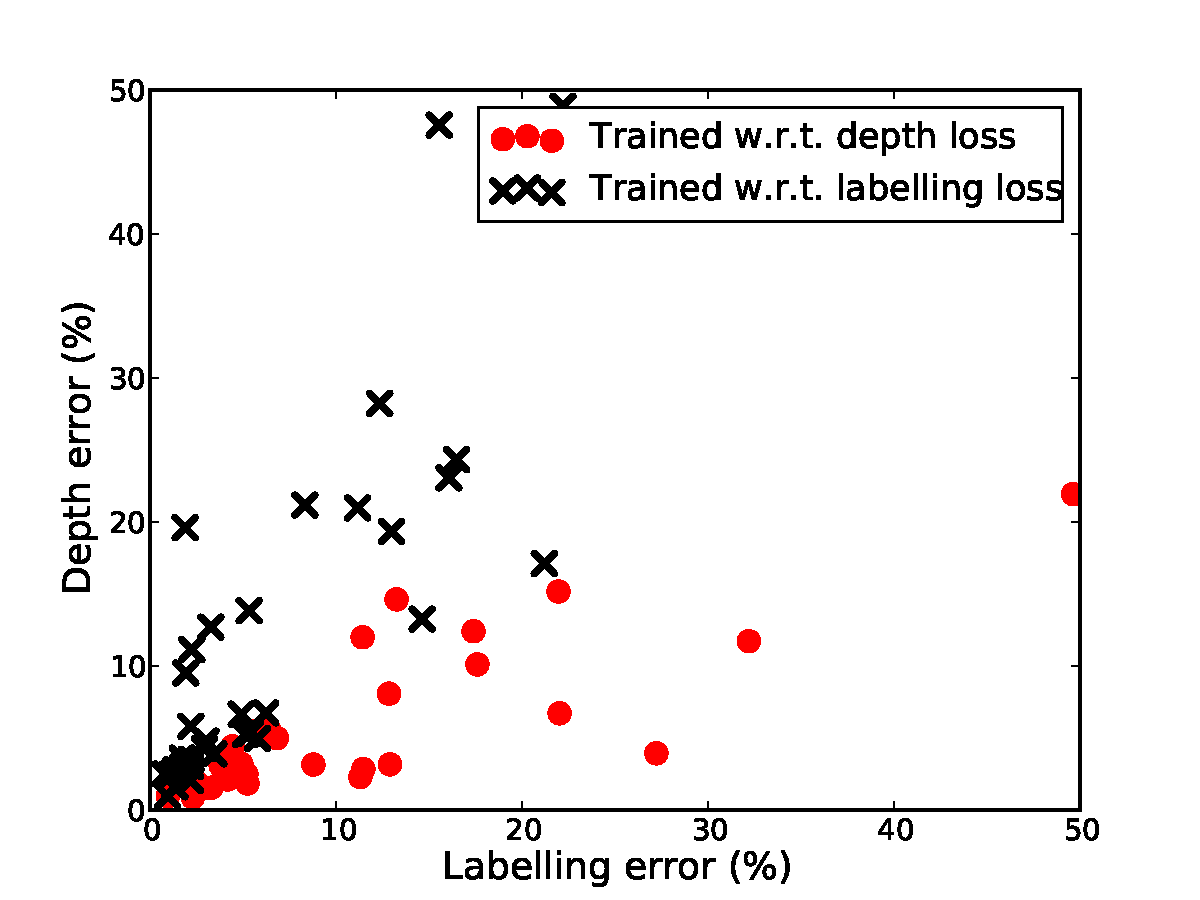
\includegraphics[width=0.6\textwidth]{comparative_scatter}
  \caption{The effect of the loss function on training. We train two
    predictors, one with respect to $\DepthLoss$ and one with respect
    to $\LblLoss$, then evaluate both on all held--out instances. Each
    data point shows the error obtained by one predictor on one held--out
    instance. The differing distribution of errors shows that the two
    predictors trade off errors as expected.}
  \label{fig:comparative-scatter}
\end{figure}

\begin{figure}[tb]
  \centering
  \subfloat[Evolution of $\Fmviewdepth$ during training]{
    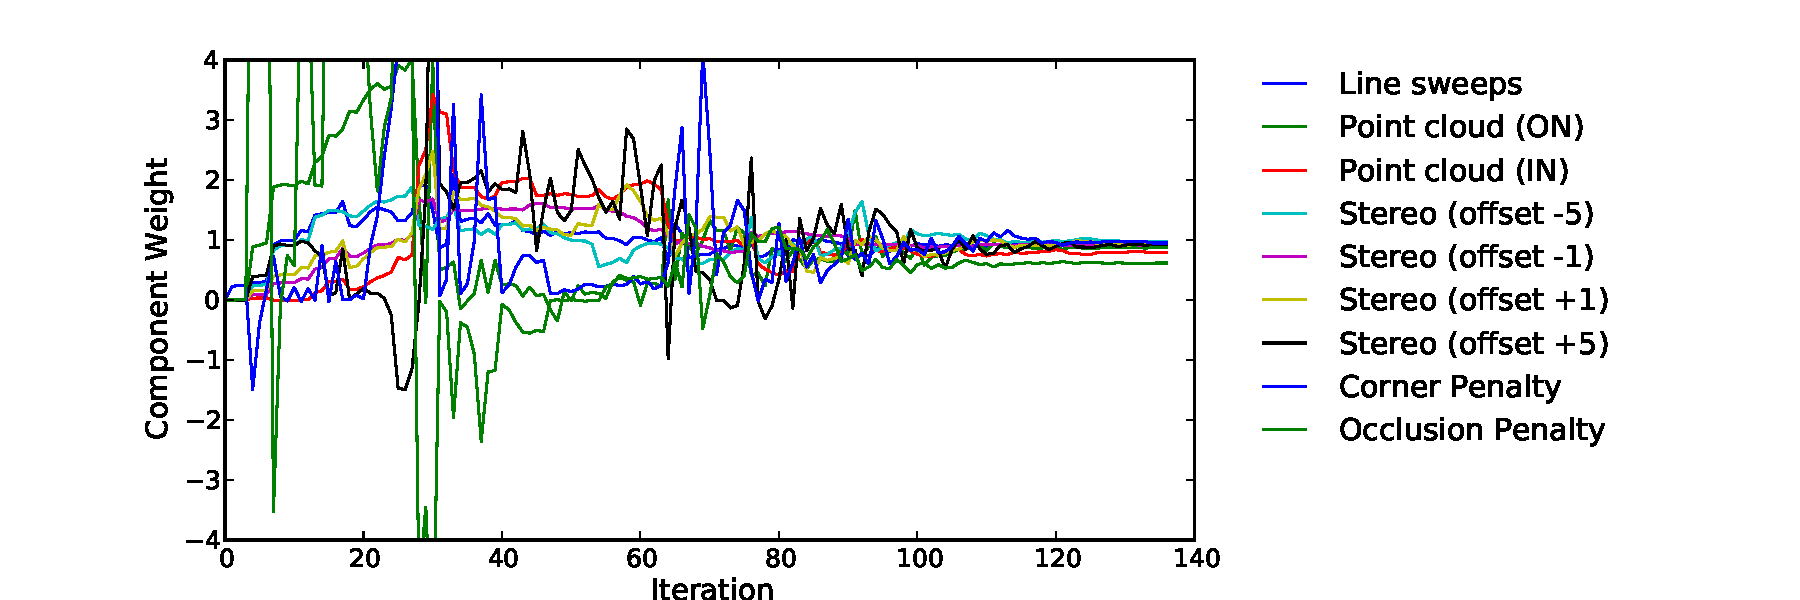
\includegraphics[width=0.8\textwidth]{psi_evolution_mview_depth}
  }
  \\
  \subfloat[Evolution of $\Fmviewlbl$ during training]{
    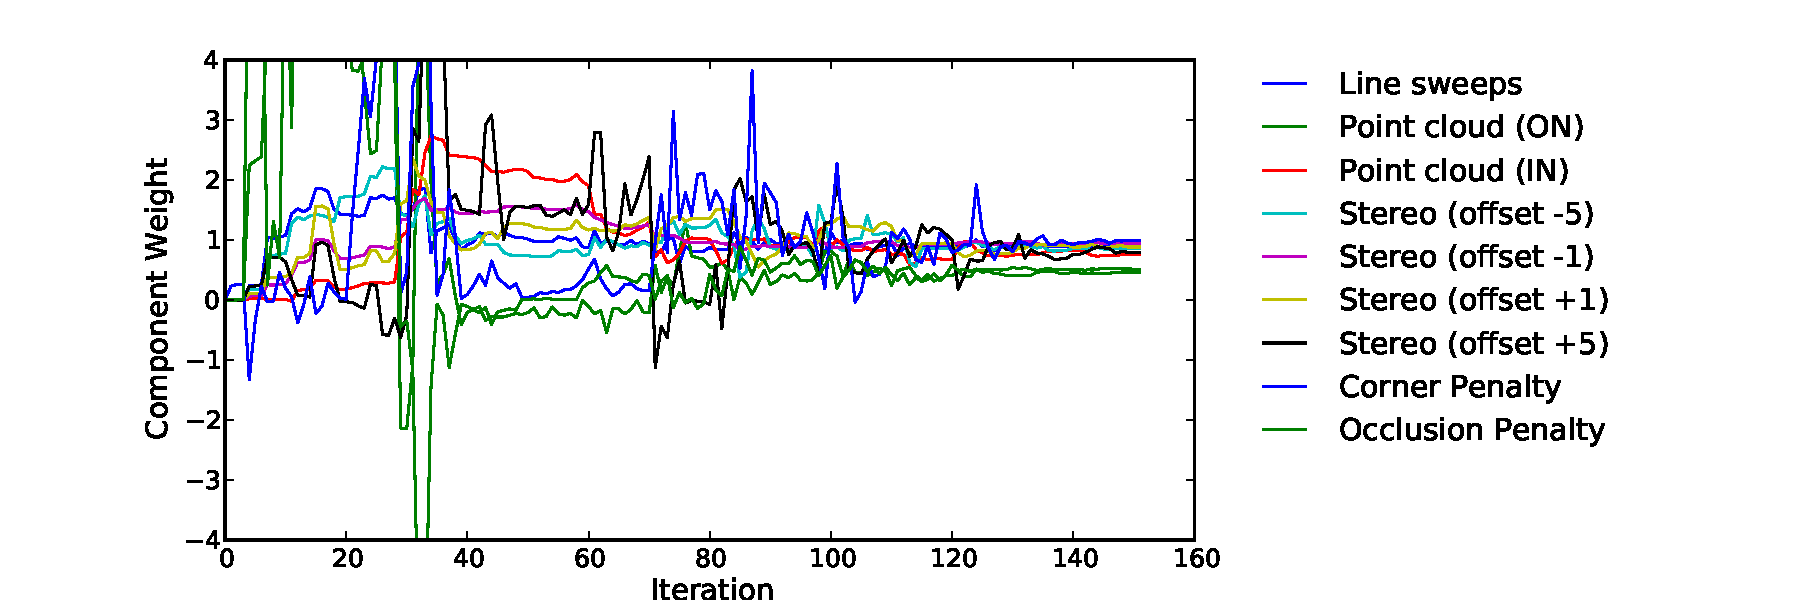
\includegraphics[width=0.8\textwidth]{psi_evolution_mview_lbl}
  }
  \\
  \subfloat[Evolution of $\Fsviewdepth$ during training (selected
    features only)]{
    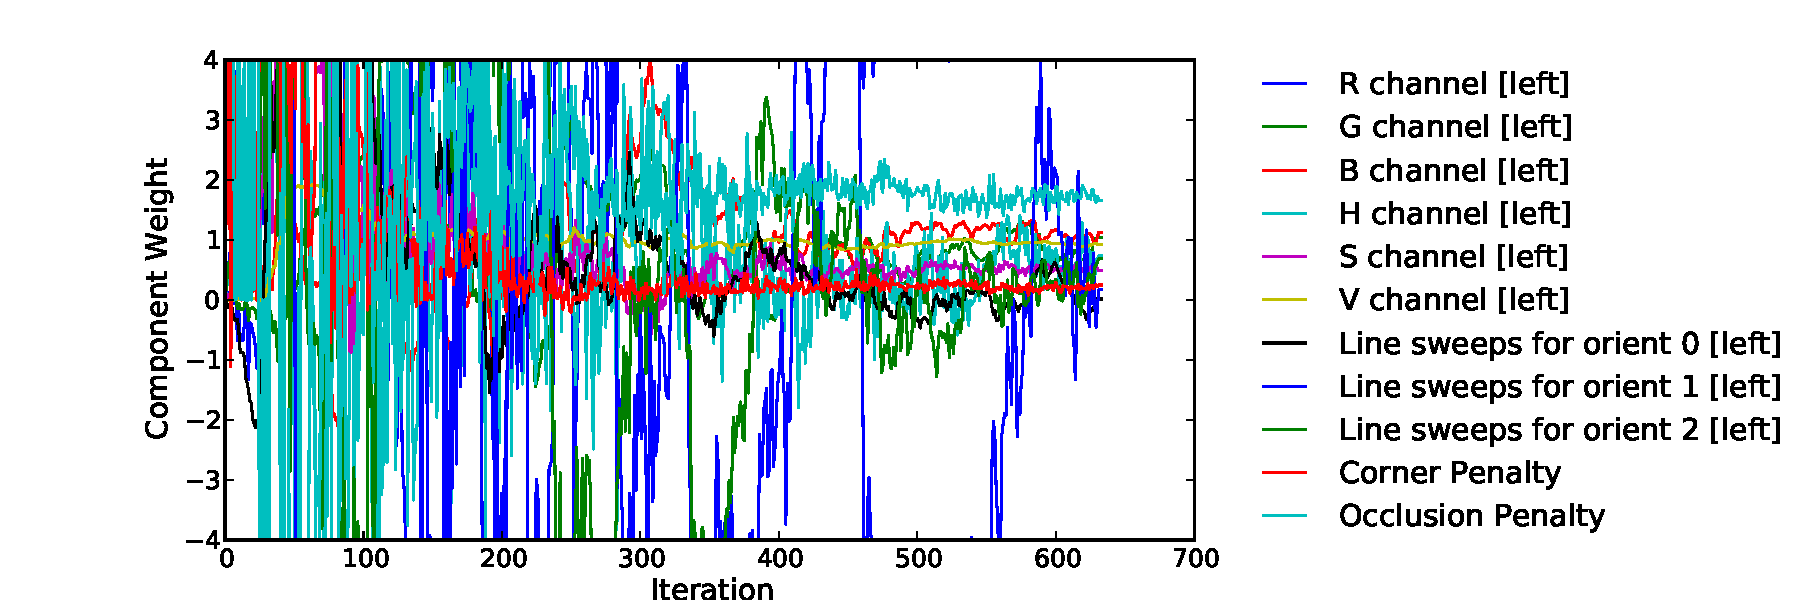
\includegraphics[width=0.8\textwidth]{psi_evolution_sview_depth}
  }
  \\
  \subfloat[Evolution of $\Fsviewlbl$ during training (selected
    features only)]{
    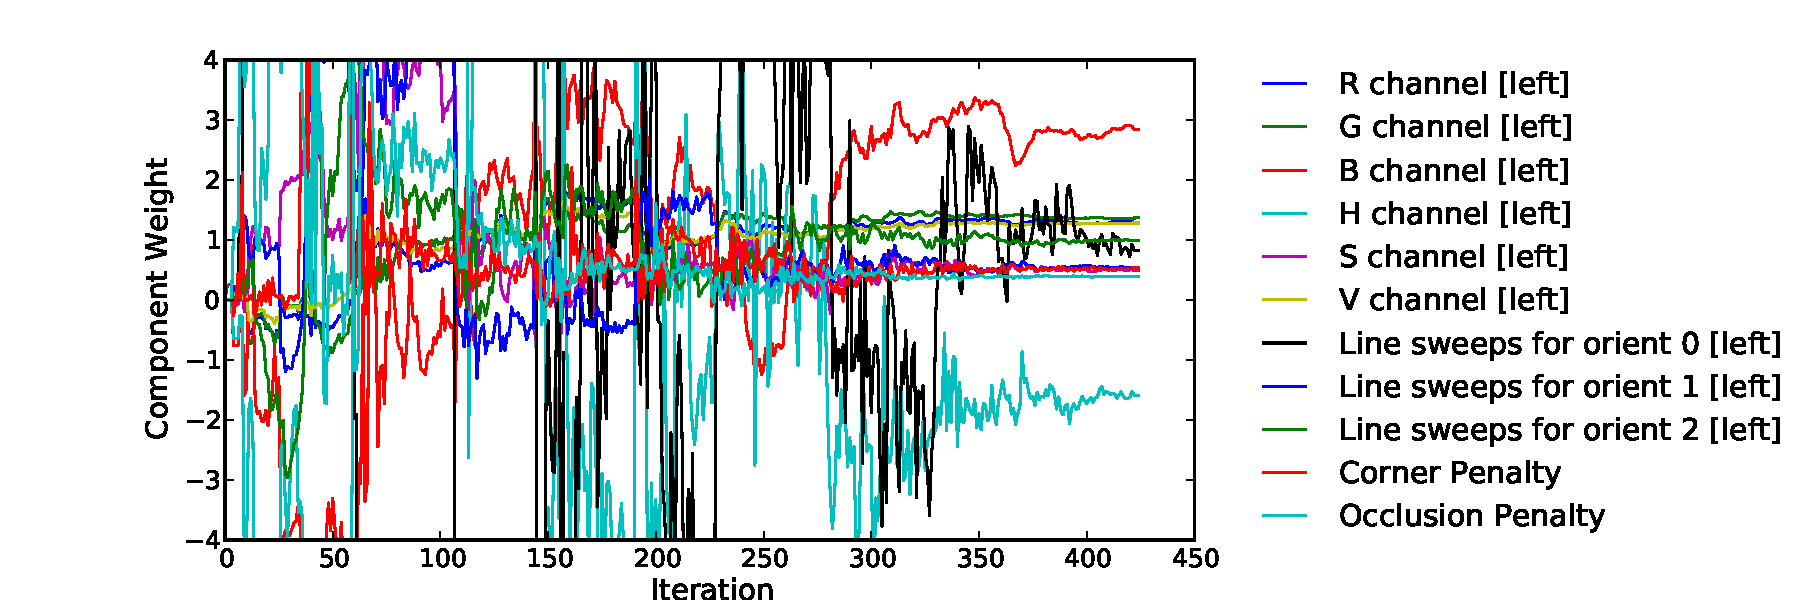
\includegraphics[width=0.8\textwidth]{psi_evolution_sview_lbl}
  }
  \caption{Evolution of model weights $\Model$ during training of each
    predictor. See main text for description of the four predictors we
    trained.}
  \label{fig:psi-evolution}
\end{figure}

\section{Single View Results}
\label{sec:sv-results}

We evaluated our system for single--view reconstruction using the same
data--set described in the previous section. We used the single--view
features summarised in \figref{featurespace}. We compared our approach
to the single--view approach described in the previous chapter and in
\cite{Flint10eccv}, which uses only line--sweep features.

Performance for each algorithm is summarised in
\tableref{learning-performance}. When measured by labelling error, our
approach out--performs the comparison system, but on the depth error
metric our approach is inferior. While investigating this result we
found that our learning algorithm assigns small weights to all but the
line--sweep features, which are the same features used by the
single--view--only instantiation of \chapref{inference}. This suggests
that the hand--tuned weights are in fact close to optimal within this
feature space, though one would expect that with additional feature
engineering our learning algorithm would be able to leverage more
salient information and reduce the error rate further.

The evolution of the weight vector $\Model$ over the course of
training is shown in \figref{psi-evolution}. Due to the size of the
single view feature space we show selected features only. The
single view learning problem is, as expected, the more difficult
problem, as shown by the considerably longer training times and the
higher volatility during the exploration phase.

\newcommand{\ExtCompFrame}[3]{ \includegraphics[width=0.18\textwidth]
  {extra_comparison_frames/#1_frame#2_#3.jpg} }

\newcommand{\MviewRow}[2]{
  \ExtCompFrame{#1}{#2}{mview_depth} &
  \ExtCompFrame{#1}{#2}{mview_lbl} &
  \ExtCompFrame{#1}{#2}{iccv} &
  \ExtCompFrame{#1}{#2}{gt}
}

\newcommand{\SviewRow}[2]{
  \ExtCompFrame{#1}{#2}{sview_depth} &
  \ExtCompFrame{#1}{#2}{sview_lbl} &
  \ExtCompFrame{#1}{#2}{eccv} &
  \ExtCompFrame{#1}{#2}{gt}
}

\begin{centering}
  \begin{longtable}{cccc}
    \caption{Reconstructions predicted by our system using the
      multiple view feature space; comparison with the bootstrapping
      approach described in \chapref{inference} and in
      \cite{Flint11}. The first two columns correspond to the
      predictors trained on $\DepthLoss$ and $\LblLoss$ respectively,
      the third column is from \chapref{inference}, and the fourth column
      is ground truth. This figure shows samples from the hold--out
      set, and were selected uniformly at random for inclusion
      here.}\\

    $\Fmviewdepth$ & $\Fmviewdepth$ & \chapref{inference} & Ground Truth \\
    \endfirsthead

    $\Fmviewdepth$ & $\Fmviewdepth$ & \chapref{inference} & Ground Truth \\
    \endhead

    \multicolumn{4}{r}{Continued on next page} \\
    \endfoot
    \endlastfoot

    \MviewRow{lab_kitchen1}{002} \\
    %\MviewRow{lab_kitchen1}{012} \\
    \MviewRow{lab_kitchen1}{022} \\
    %\MviewRow{lab_kitchen1}{032} \\
    \MviewRow{lab_kitchen1}{042} \\
    %\MviewRow{lab_kitchen1}{052} \\
    \MviewRow{lab_kitchen1}{062} \\
    %\MviewRow{lab_kitchen1}{072} \\
    \MviewRow{lab_kitchen1}{082} \\
    %\MviewRow{lab_kitchen1}{092} \\

    %\MviewRow{exeter_mcr1}{002} \\
    \MviewRow{exeter_mcr1}{012} \\
    %\MviewRow{exeter_mcr1}{022} \\
    \MviewRow{exeter_mcr1}{032} \\
    %\MviewRow{exeter_mcr1}{042} \\
    \MviewRow{exeter_mcr1}{052} \\

    %\MviewRow{lab_foyer1}{002} \\
    \MviewRow{lab_foyer1}{012} \\
    %\MviewRow{lab_foyer1}{022} \\
    \MviewRow{lab_foyer1}{032} \\
    %\MviewRow{lab_foyer1}{042} \\

    %\MviewRow{lab_foyer2}{002} \\
    \MviewRow{lab_foyer2}{012} \\
    %\MviewRow{lab_foyer2}{022} \\
    \MviewRow{lab_foyer2}{032} \\
    \MviewRow{lab_foyer2}{042} \\

    %\MviewRow{som_corr1}{012} \\
    \MviewRow{som_corr1}{022} \\
    %\MviewRow{som_corr1}{032} \\
    \MviewRow{som_corr1}{042} \\

    %\MviewRow{lab_ground1}{002} \\
    \MviewRow{lab_ground1}{012} \\
    %\MviewRow{lab_ground1}{022} \\
    \MviewRow{lab_ground1}{032} \\
    %\MviewRow{lab_ground1}{042} \\
  \end{longtable}
  \label{fig:mview-outputs}
\end{centering}


\begin{centering}
  \begin{longtable}{cccc}
    \caption{Reconstructions predicted by our system using the single
      view feature space; comparison with the bootstrapping approach
      described in \chapref{inference} and in \cite{Flint11}. The
      first two columns correspond to the predictors trained on
      $\DepthLoss$ and $\LblLoss$ respectively, the third column is
      from \chapref{inference} using photometric featues alone, and
      the fourth column is ground truth. This figure shows samples
      from the hold--out set, and were selected uniformly at random
      for inclusion here.}\\

    $\Fsviewdepth$ & $\Fsviewdepth$ & \chapref{inference} & Ground Truth \\
    \endfirsthead

    $\Fsviewdepth$ & $\Fsviewdepth$ & \chapref{inference} & Ground Truth \\
    \endhead

    \multicolumn{4}{r}{Continued on next page} \\
    \endfoot
    \endlastfoot

    %\SviewRow{lab_kitchen1}{002} \\
    \SviewRow{lab_kitchen1}{012} \\
    %\SviewRow{lab_kitchen1}{022} \\
    \SviewRow{lab_kitchen1}{032} \\
    %\SviewRow{lab_kitchen1}{042} \\
    \SviewRow{lab_kitchen1}{052} \\
    %\SviewRow{lab_kitchen1}{062} \\
    \SviewRow{lab_kitchen1}{072} \\
    %\SviewRow{lab_kitchen1}{082} \\
    \SviewRow{lab_kitchen1}{092} \\

    %\SviewRow{exeter_mcr1}{002} \\
    \SviewRow{exeter_mcr1}{012} \\
    %\SviewRow{exeter_mcr1}{022} \\
    \SviewRow{exeter_mcr1}{032} \\
    %\SviewRow{exeter_mcr1}{042} \\
    \SviewRow{exeter_mcr1}{052} \\

    %\SviewRow{lab_foyer1}{002} \\
    \SviewRow{lab_foyer1}{012} \\
    %\SviewRow{lab_foyer1}{022} \\
    \SviewRow{lab_foyer1}{032} \\
    %\SviewRow{lab_foyer1}{042} \\

    %\SviewRow{lab_foyer2}{002} \\
    \SviewRow{lab_foyer2}{012} \\
    %\SviewRow{lab_foyer2}{022} \\
    \SviewRow{lab_foyer2}{032} \\
    %\SviewRow{lab_foyer2}{042} \\

    %\SviewRow{som_corr1}{012} \\
    \SviewRow{som_corr1}{022} \\
    %\SviewRow{som_corr1}{032} \\
    \SviewRow{som_corr1}{042} \\

    %\SviewRow{lab_ground1}{002} \\
    \SviewRow{lab_ground1}{012} \\
    %\SviewRow{lab_ground1}{022} \\
    \SviewRow{lab_ground1}{032} \\
    %\SviewRow{lab_ground1}{042} \\
  \end{longtable}
  \label{fig:sview-outputs}
\end{centering}


\section{Discussion}
\label{sec:discussion}

The hypothesis class considered in this chapter is amongst the most
complex (in terms of internal constraints on the output space) studied
within the structured prediction framework. In this section we turn to
some practical lessons learned that may be of value to other
practitioners.

\subsection{Condition in the joint feature space, not the input
  feature space.}

A common pre--processing operation for statistical learning is to
transform the observed features $\Features$ to zero mean and unit
variance. However, for structured prediction tasks it is the joint
feature space $\JointFtr$, not the input feature space, that should be
conditioned:
\begin{equation}
  \label{eq:conditioning}
  \JointFtr' = \frac{\JointFtr - \mu}{\sigma^2} ~.
\end{equation}
Ideally one would sample directly from the joint feature space to
determine the conditioning transformation, but the distribution of
inputs and outputs is generally unknown in an empirical risk
minimisation setting. Instead, we suggest using the training set as a
proxy. We compute the empirical mean and variance of
$\{\JointFtr(\Features_k,\Seam_k)\}_{k=1}^n$ for the training set at
the outset, then apply the transformation \eqnref{conditioning} after
each feature computation.

\subsection{Condition the loss terms.}

For any $\eta>0$, the minimisation problem \eqnref{svm-problem} is
equivalent to the following (this is proved in Proposition
\ref{prop:equivalence} at the end of this chapter):
\begin{equation}
  \begin{split}
    \min_{\Model',\Slacks'} &
      \hspace{2mm} 
    \frac{1}{2} \|\Model'\|^2 +
      \eta C \sum_{k=1}^n \Slack_k'\\
    s.t. & \hspace{2mm} \forall k, \Seam \neq \Seam_k:~
      \bigl\langle\Model', \JointFtr(\Features_k,\Seam_k)\bigr\rangle -
      \bigl\langle\Model', \JointFtr(\Features_k,\Seam)\bigr\rangle
      \geq
      %%% TODO: in the line below 1/eta should be replaced with eta --
      %%% this was incorrect in the review submission!!
      \eta \Loss(\Seam,\Seam_k) - \Slack_k' ~.
  \end{split}
  \label{eq:equiv-problem}
\end{equation}
Although any $\eta>0$ preserves the correctness of the optimisation
algorithm, we found that choosing $\eta=\mbox{Var}(\Loss)$ improved
numerical stability, since this means that the loss terms will have
roughly unit variance. Unfortunately, we cannot use the training set
to estimate $\mbox{Var}(\Loss)$ since the loss for the ground truth
output is always zero. Instead we computed
$\Loss(\Features_k,\Seam_j)$ for each $k \neq j$ in the training
set. This is not an ideal estimate, but we found that it worked well
in practice.

\subsection{Check that the hypothesis class contains the ground
  truth.}

The algorithm described in \cite{Tsochantaridis04} implicitly assumes
that the hypothesis class $\mathcal{Y}$ contains the ground truth
labels $\Seam_k$. This means that if $\AugSeam$ is the maximiser of
\eqnref{separation-problem} then
\begin{equation}
  \bigl\langle\Model, \JointFtr(\Features_k,\Seam_k)\bigr\rangle
  - \bigl\langle\Model, \JointFtr(\Features_k,\AugSeam)\bigr\rangle
  - \Loss(\AugSeam,\Seam_k) 
  \leq 
  0 ~,
  \label{eq:positive-slacks}
\end{equation}
since otherwise we would have
\begin{equation}
  \bigl\langle\Model, \JointFtr(\Features_k,\Seam_k)\bigr\rangle
  + \Loss(\Seam_k,\Seam_k) 
  >
  \bigl\langle\Model, \JointFtr(\Features_k,\AugSeam)\bigr\rangle
  + \Loss(\AugSeam,\Seam_k) ~,
\end{equation}
contradicting $\AugSeam$ as the maximiser of
\eqnref{separation-problem}. However, our output space contains
fundamentally real--valued quantities such as polygon vertices, which
are recovered only to some finite precision by the inference
algorithm, and since our ground truth labels were acquired by manual
labelling, they sometimes exceed the maximum precision of the
inference algorithm. In this case we effectively have $\Seam_k \notin
\mathcal{Y}$ (although there is always some $\Seam' \in \mathcal{Y}$
close to $\Seam_k$), so it is possible that $\AugSeam$ violates
\eqnref{positive-slacks}. Our workaround here is simply to check the
condition \eqnref{positive-slacks} each time we solve the separation
problem and, if violated, substitute $\Seam_k$ for $\AugSeam$. This is
justified by the observation that if \eqnref{positive-slacks} is
violated for $\AugSeam$ then it is violated for all
$\Seam\in\mathcal{Y}$. One could think of this as learning with
respect to the hypothesis class $\mathcal{Y} \union \{\Seam_k\}$ but
evaluating with respect to $\mathcal{Y}$. Again, this is not an ideal
solution but we found it to work well in practice.

%\newcommand{\CompFrame}[3]{
%  \includegraphics[width=0.18\textwidth]
%                  {comparison_frames/#1_frame#2_#3.png}
%}

%% \begin{figure}[tb]%
%%   \centering
%%   \begin{tabular}{cccccc}
%%     \begin{sideways}
%%       $~~~\DepthLoss$
%%     \end{sideways} &
%%     \CompFrame{lab_foyer1}{002}{depthtrained} &
%%     \CompFrame{lab_ground1}{012}{depthtrained} &
%%     \CompFrame{exeter_mcr1}{012}{depthtrained} &
%%     \CompFrame{exeter_mcr1}{042}{depthtrained} &
%%     \CompFrame{som_corr1}{022}{depthtrained} 
%%     \\

%%     \begin{sideways}
%%       $~~~\LblLoss$
%%     \end{sideways} &
%%     \CompFrame{lab_foyer1}{002}{lbltrained} &
%%     \CompFrame{lab_ground1}{012}{lbltrained} &
%%     \CompFrame{exeter_mcr1}{012}{lbltrained} &
%%     \CompFrame{exeter_mcr1}{042}{lbltrained} &
%%     \CompFrame{som_corr1}{022}{lbltrained} 
%%     \\

%%     \begin{sideways}
%%       Flint \etal
%%     \end{sideways} &
%%     \CompFrame{lab_foyer1}{002}{iccv} &
%%     \CompFrame{lab_ground1}{012}{iccv} &
%%     \CompFrame{exeter_mcr1}{012}{iccv} &
%%     \CompFrame{exeter_mcr1}{042}{iccv} &
%%     \CompFrame{som_corr1}{022}{iccv} 
%%     \\

%%     \begin{sideways}
%%       $~~$Ground
%%     \end{sideways}
%%     \begin{sideways}
%%       $~~~$Truth
%%     \end{sideways} &
%%     \CompFrame{lab_foyer1}{002}{gt} &
%%     \CompFrame{lab_ground1}{012}{gt} &
%%     \CompFrame{exeter_mcr1}{012}{gt} &
%%     \CompFrame{exeter_mcr1}{042}{gt} &
%%     \CompFrame{som_corr1}{022}{gt} 
%%   \end{tabular}
%%   \caption{Multiple--view reconstructions predicted by our system
%%     (held--out samples). The first two rows represent the
%%     predictors trained on $\DepthLoss$ and $\LblLoss$ respectively,
%%     the third row is from \cite{Flint11}, and the fourth row is ground
%%     truth.}
%%   \label{fig:mv-results-egs}
%% \end{figure}

\subsection{Equivalence of \eqnref{svm-problem} and \eqnref{equiv-problem}}
\label{sec:equivalence-proof}

Here we prove the equivalence of the minimisation problems
\eqnref{svm-problem} and \eqnref{equiv-problem} stated above. For
clarity we re--state the claim in the following proposition.

\begin{proposition}
\label{prop:equivalence}
  Let $\Model,\Slacks$ be the solution to
  \begin{equation}
    \begin{split}
      \min_{\Model,\Slacks} &
      \hspace{2mm} 
      \frac{1}{2} \|\Model\|^2 +
      C \sum_{k=1}^n \Slack_k\\
      s.t. & \hspace{2mm} \forall k, \Seam \neq \Seam_k:~
      \bigl\langle\Model, \JointFtr(\Features_k,\Seam_k)\bigr\rangle -
      \bigl\langle\Model, \JointFtr(\Features_k,\Seam)\bigr\rangle
      \geq
      \Loss(\Seam,\Seam_k) - \Slack_k ~.
    \end{split}
    \label{eq:svm-problem2}
  \end{equation}
  Let $\Model',\Slacks'$ be the solution to
  \begin{equation}
    \begin{split}
      \min_{\Model',\Slacks'} &
      \hspace{2mm} 
      \frac{1}{2} \|\Model'\|^2 +
      \eta C \sum_{k=1}^n \Slack_k'\\
      s.t. & \hspace{2mm} \forall k, \Seam \neq \Seam_k:~
      \bigl\langle\Model', \JointFtr(\Features_k,\Seam_k)\bigr\rangle -
      \bigl\langle\Model', \JointFtr(\Features_k,\Seam)\bigr\rangle
      \geq
      \eta \Loss(\Seam,\Seam_k) - \Slack_k' ~.
    \end{split}
    \label{eq:equiv-problem2}
  \end{equation}
  Then
  \begin{eqnarray}
    \Model' &=& \eta \Model\\
    \Slacks' &=& \eta \Slacks ~.
  \end{eqnarray}
\end{proposition}
\begin{proof}
  Substituting for $\Model'$ and $\Slacks'$ in \eqnref{equiv-problem2},
  \begin{equation}
    \begin{split}
      \min_{\Model,\Slacks} &
      \hspace{2mm} 
      \frac{1}{2} \| \eta \Model \|^2 +
      \eta C \sum_{k=1}^n \eta \Slack_k\\
      s.t. & \hspace{2mm} \forall k, \Seam \neq \Seam_k:~
      \bigl\langle\eta\Model, \JointFtr(\Features_k,\Seam_k)\bigr\rangle -
      \bigl\langle\eta\Model, \JointFtr(\Features_k,\Seam)\bigr\rangle
      \geq
      \eta \Loss(\Seam,\Seam_k) - \eta\Slack_k
    \end{split}
    \label{eq:problem2}
  \end{equation}
  and dividing the objective by $\eta^2$ and the constraints by $\eta$
  we obtain the desired result.
\end{proof}

\section{Conclusion}
\label{sec:conclusion}

We have presented a unified learning framework for recovering
semantically meaningful geometric models from single and multiple
views of a scene. We have chosen to work with the indoor Manhattan
class in order to leverage the simple parametrisation and efficient
inference algorithm made possible by this hypothesis class. Our
approach to learning performs a single optimisation with respect to a
clearly defined loss function. Experiments show our system
out--performing the approach of the previous chapter in the
multiple--view setting (by a large margin) and on one metric in the
single--view setting.
